\bichapter{绪论}{introduction}

\bisection{研究目的及意义}{Purpose and significance of the study}

纳米零价铁(NZVI)因为独特的物理和化学性质,如高界面反应性显示出在处理废水中有机污染物方面具有巨大潜力;极小的粒径使NZVI可以直接注入受污染的含水层中\cite{2}。因此NZVI越来越多地用于污染土壤和含有氯化溶剂和重金属的地下水的原位修复\cite{1,WOS:000704630800008,REN2022127322,LI201916}。然而,研究表明,纳米零价铁在实验室研究和现场试验中的迁移性和稳定性表现均不理想\cite{3}。主要原因在于分散在水相中的纳米零价铁颗粒由于磁力作用而具有强烈的聚集趋势,形成远超过微米尺寸的枝状絮体和网状结构,降低了它的有效表面积和反应活性\cite{4},以及NZVI的高表面活性导致其常在与污染物接触前被氧化,于表面形成铁氧化物外壳,导致NZVI活性降低\cite{HUANG2016168}。同时,砂粒表面在中性条件下带负电,零价铁颗粒易吸附在其表面上\cite{5},使得零价铁在多孔介质中不易扩散。因此研究纳米零价铁在多孔介质中的迁移,增强纳米铁的稳定性与分散性,提高其在介质中的迁移距离,对实现 NZVI 颗粒在可操作条件下成功运送至“反应区域”具有重要意义。

\bisection{纳米零价铁的研究现状}{NZVI}

零价铁(Zero-Valent Iron,ZVI)由于具有很强的还原能力(E0 = -0.44 V)和吸附重金属、金属等一系列重要污染物的能力,在环境修复中得到了广泛的研究\cite{6}。Gould\cite{7}报道了ZVI在环境中的最早应用,他研究了金属铁丝还原六价铬的动力学。使用纳米零价铁(Nano Zero-Valent Iron, NZVI)在地下进行原位脱氯的概念首先由Wang和Zhang\cite{8}提出,他们假设nZVI可以直接注入受污染的地下水中,并有助于污染土壤和地下水的原位修复\cite{1}。Wang和Zhang\cite{8}证明了合成的、不稳定的ZVI颗粒用于还原脱氯的有效性,并指出新制备的ZVI颗粒比商业铁粉的活性高得多。Zhang等\cite{9}还报道了添加少量催化剂(Pd)可使表面积归一化速率常数增加约100倍。然而所有这些开创性的工作都是在水溶液中进行的,并没有解决与土壤修复相关的其他关键问题,如nZVI易钝化、易流失、颗粒易聚集,土壤输送能力差等。随后,技术进入了一个强调颗粒稳定和迁移性的新阶段。

nZVI的稳定化可以通过表面改性和(或)创建分离纳米粒子的网络来实现,如\cref{fig1}所示。nZVI的稳定剂可分为表面活性剂、合成或天然大分子或高分子电解质、粘度调节剂、油乳化剂和微尺度固体载体。 

\begin{figure}[h]
    \begin{subfigure}{.5\textwidth}
		\centering
		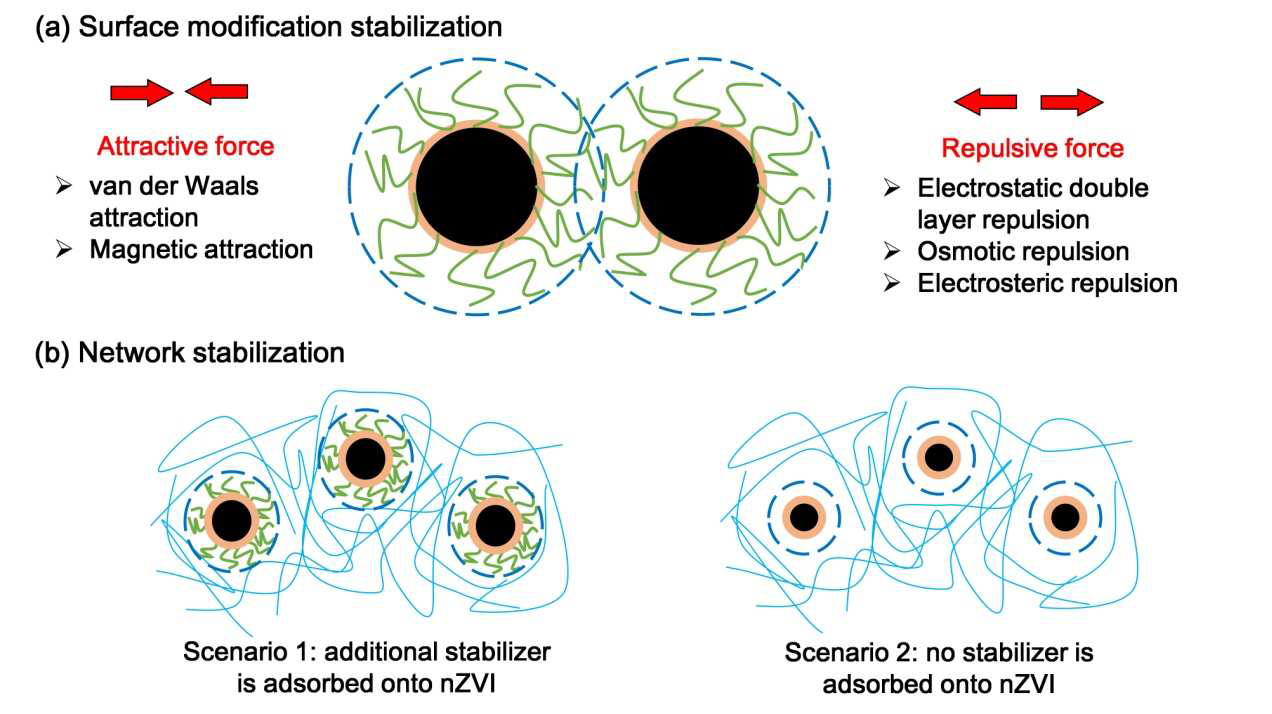
\includegraphics[width=\textwidth]{figs/fig1.png}
	\end{subfigure}
    
	\begin{subfigure}{.5\textwidth}
		\centering
		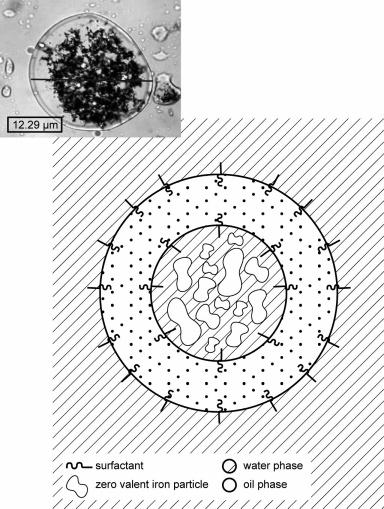
\includegraphics[width=\textwidth]{figs/fig2.png}
	\end{subfigure}
    \bicaption{(a)纳米零价铁稳定化示意图(b)EZVI液滴示意图}{(a)Schematic diagram of stabilized NZVI (b)Schematic diagram of EZVI droplets}\label{fig1}
\end{figure}

硫化纳米零价铁(Sulfidated Nanoscale Zero Valent Iron, S-NZVI)是一种对 NZVI 进行表面钝化的改性方法,在原有的零价铁内核-氧化物外壳结构的基础上,再形成了一层铁硫化物的外壳($\mathrm{FeS_x}$),该$\mathrm{FeS_x}$保护层可以有效的防止内层的NZVI内核被周围环境介质氧化\cite{doi:10.1021/acs.est.8b01735}。此外,$\mathrm{FeS_x}$保护层内存在的离域电子有助于电子传递的进行,因此提高了材料对污染物的还原能力,很好地解决了NZVI易钝化的缺点\cite{doi:10.1021/acs.est.8b01735,doi:10.1021/acs.est.6b03997,15}。Kim等\cite{16}发现,硫化条件下形成的纳米零价铁双相材料(Fe/FeS),比仅与氧化铁(Fe/FeO)结合的nZVI更快地还原三氯乙烯(TCE),并且将Fe/FeS暴露于溶解有$\mathrm{Pd}^{2+}$、$\mathrm{Cu}^{2+}$、$\mathrm{N}^{2+}$、$\mathrm{Co}^{2+}$和$\mathrm{Mn}^{2+}$的溶液中可以进一步提高脱氯反应性。然而,由于纳米颗粒的范德华力和零价铁的磁性作用,S-nZVI颗粒仍然会形成团聚体,这大大减少了它们在受污染的地下水中的传输。因此需要对S-NZVI颗粒进行改性,引入克服范德华力和磁性的斥力,以增强S-NZVI的稳定性,从而增强其在地下水中的迁移能力。

表面活性剂是常用的控制颗粒之间的相互作用的稳定剂之一。张永祥、马晓敏等\cite{10}以聚乙二醇( PEG) 为分散剂,在乙醇-水混合溶剂中合成改性纳米零价铁(NZVI)颗粒,讨论了nZVI去除Cr(VI)的影响因素,并对反应产物进行XPS检测。结果表明,乙醇比例为50\%时制备出的纳米零价铁直径在30~60 nm,对Cr(VI)的去除率最高,为95.30\%。NZVI投加量越大,Cr(VI)初始浓度越小,pH越小,温度越高,均有利于水中Cr(VI)的去除。纳米零价铁将Cr(VI)吸附后将其还原为Cr(III),反应过程主要以还原作用为主。

% 目前已有大量关于包覆型NZVI分散性能的研究,基于DLVO理论测定颗粒的$\zeta$电位计算双电层斥力和范德华力,考虑了包覆层提供的空间作用力分析颗粒的稳定效果\cite{doi:10.1080/09593330.2018.1426637},但是考虑包覆层对颗粒表面电荷的影响的研究较少。对于包覆型NZVI,聚合物吸附固定于颗粒表面形成吸附层,同时溶液中的阴阳离子可以穿透软粒子表面,电荷可以分布在颗粒表面和吸附层内部,因此颗粒的电泳迁移率同时受到颗粒表面电势、Donnan电势及带电聚合物的影响\cite{WOS:000692041500001}。因此软粒子的电泳迁移率对滑移面不敏感,$\zeta$电位失去意义,基于硬粒子假设的Smoluchowski理论并不适用\cite{OHSHIMA20152,Ohshima1995}。

% 本文使用海藻酸钠包覆S-NZVI,防止聚集和沉降,提升在地下水中的迁移能力。阴离子聚电解质的使用与颗粒在地下水的流动性相关,因为在地下水中遇到的大多数矿物和天然有机物表面都带负电\cite{YU2020111245,WOS:000243124600047}。因此,阴离子聚电解质包覆层能够提供来自这些表面的静电斥力,以减少粘附现象。利用动态光散射(DLS)测定颗粒的尺寸,计算团聚速率结合沉降实验,评价颗粒的稳定性。使用Ohshima的软粒子理论计算包覆型S-NZVI的表面电势及包覆层的厚度和软度,结合扩展DLVO理论,解释包覆型S-NZVI的团聚机理,利用Smoluchowski团聚动力学模型预测颗粒平均粒径随时间的变化曲线。最后进行柱实验研究不同注入速度和注入浓度对纳米铁在多孔介质中迁移的影响。将颗粒粒径变化带入迁移计算中,预测不同条件下纳米铁再迁移柱中的最大迁移距离。

与表面活性剂相比,合成聚合物和天然聚合物材料已经被更广泛地研究\cite{ZHOU2014155}。聚电解质通过吸附接枝的方式固定于NZVI颗粒表面,形成聚合物包覆层,层内的大分子为包覆粒子提供静电斥力和空间斥力\cite{2018Impact,doi:10.108007388551.2018.1440525}避免其发生团聚。此外,这些大分子不仅能有效地促进NZVI的稳定,还能被微生物降解,作为微生物群落的能量来源。张永祥、常杉等\cite{11} 利用羧甲基淀粉钠(CMS)对nZVI进行包覆改性,利用空间位阻效应提高其分散悬浮性。研究其对2,4-二氯苯酚(2,4-DCP)的去除效果。结果表明,改性后的nZVI直径大约在80~100 nm,呈链状或分散颗粒分布,主要物质组成为零价铁,具有强还原性。当CMS的比例为80.00\%时,悬浮性最佳;经过CMS包覆改性后,nZVI还保留原有的活性,在不同包覆比例对于2,4-DCP的去除效果的实验中发现,同样CMS比例为80\%时去除效果最好,达到83.69\%,且有明显的脱氯降解过程。

乳化型纳米铁的开发是为了针对地下水中高密度非水相液体(Dense nonaqueous-phase liquids,DNPLs)的去除。通常使用食品级表面活性剂、可生物降解的植物油和水将nZVI包装成油滴,即使用油膜包围nZVI,然后疏水油膜涂层使DNAPL浓缩,nZVI将其降解\cite{12},如\cref{fig1}所示。

负载型纳米铁是将微尺度的固体材料作为载体或是支撑材料来稳定nZVI。张永祥、王友好等\cite{13, 14} 研究新制备复合材料改性沸石负载纳米零价铁/镍去除水中2,4-二氯苯酚效果以及该材料在地下水污染原位修复中的应用情况,开展了2,4-二氯苯酚的批实验和柱实验。批实验结果表明, 25℃时,0.6 g的复合材料对20 mg·L-1的2,4-DCP去除效果达到80\%;柱实验结果表明,材料的双金属颗粒分散性良好,避免了团聚现象的出现。

\bisection{纳米零价铁的注入方式}{}

nZVI的直接注入技术可概括为以下几种方法:

\begin{itemize}
    \item 通过固定注入点将nZVI泥浆引入处理区\cite{17};
    \item 通过气动或水力压裂在注入点周围形成优先流动路径的裂缝网络,并增强nZVI的分布\cite{18};
    \item 通过压力脉冲技术注入nZVI泥浆;
    \item 将nZVI流体混合物与载气相结合,形成可分散到处理区的气溶胶\cite{19};
    \item 通过重力进料注入\cite{20};
    \item 使用携带nZVI的泡沫表面活性剂注入\cite{21}。
\end{itemize}

nZVI在原位修复中的直接注入技术已经较为成熟,基本目的都是将特定量的nZVI泥浆直接注入到含水层中。He等\cite{22}在压力作用下,注入CMC稳定的Fe/Pd纳米材料,用于阿拉巴马北部含水层中四氯乙烯(PCE)、三氯乙烯(TCE)和多氯联苯(PCBs)污染物的原位治理,沿地下水流向共设置4口试验井,在长达596天的试验时间里,纳米材料有助于非生物降解的早期快速进行,长期来看,以CMC为碳源,以非生物/生物过程中的氢为电子供体,促进了现有的生物降解过程,导致了地下水中氯代有机污染物的持续强化破坏。Su等\cite{23}在美国的Parris岛进行了表面修饰型纳米铁材料的现场测试,并对其进行了两年半的监测,以评估对PCE为主的地下源区氯化挥发性有机污染物的处理效果,分别采用了气动注入和固定点注入两种方式,气动注入时能够传输2.1m,但固定点注入只能移动0.89m。Ariel等\cite{24}在加拿大萨尼亚市的一个氯化溶剂污染场地进行现场试验,采用复合改性方式,制得CMC-S-nZVI悬浮液,并通过重力注入到砂质材料中,上游和下游井中收集的样品表明铁颗粒的径向和垂直分布效果优良,行进距离0.9m-2.7m,在地下水中具有稳定的流动性,并且对场地中的多种氯化类有机污染物有着良好的反应活性。

\bisection{本文主要研究内容}{}

\subsection{SA-S-NZVI的颗粒稳定性研究}

制备不同包覆比的SA-S-NZVI并研究不同包覆比的沉降曲线;研究不同pH值S-NZVI的$\zeta$电位、不同离子强度各包覆比SA-S-NZVI的电泳迁移率和粒径变化情况,结合Ohshima的软粒子理论计算SA-S-NZVI的表面电势及包覆层的厚度和软度,结合扩展DLVO理论,解释包覆型S-NZVI的团聚机理,利用Smoluchowski团聚动力学模型预测颗粒平均粒径随时间的变化曲线。

\subsection{SA-S-NZVI在多孔介质的迁移性能研究}

通过柱实验研究SA-S-NZVI悬浮液在多孔介质中的运移过程,堵塞的形成、发展过程;堵塞对多孔介质水力特性造成的影响;纳米零价铁在多孔介质中的分布规律;深入分析造成堵塞的机理。

\subsection{技术路线}


% \begin{multline}
% \frac{1}{2}\Delta(f_{ij}f^{ij})=
% 2\left(\sum_{i<j}\chi_{ij}(\sigma_i-\sigma_j)^2+f^{ij}\nabla_j\nabla_i(\Delta f)+\right .\\
% \left .\nabla_kf_{ij}\nabla^kf^{ij}+f^{ij}f^k\left[2\nabla_iR_{jk}-\nabla_kR_{ij}\right]\vphantom{\sum_{i<j}}\right)
% \end{multline}


% 参见\cref{eq:none}:
% \begin{align}
% \label{eq:none}
% &I(X_3;X_4)-I(X_3;X_4\mid{}X_1)-I(X_3;X_4\mid{}X_2)\nonumber\\
% =&[I(X_3;X_4)-I(X_3;X_4\mid{}X_1)]-I(X_3;X_4\mid{}\tilde{X}_2)\\
% =&I(X_1;X_3;X_4)-I(X_3;X_4\mid{}\tilde{X}_2)
% \end{align}

% \begin{figure}[!htp]
% 	\centering
% 	\resizebox{10cm}{!}{\usetikzlibrary{shapes.geometric, arrows}
\tikzstyle{startstop} = [
rectangle,
rounded corners,
minimum width=2cm,
minimum height=1cm,
text centered,
draw=black
]
\tikzstyle{io} = [
trapezium,
trapezium left angle=75,
trapezium right angle=105,
minimum width=1cm,
minimum height=1cm,
text centered,
draw=black
]
\tikzstyle{process} = [
rectangle,
minimum width=2cm,
minimum height=1cm,
text centered,
draw=black
]
\tikzstyle{decision} = [
diamond,
minimum width=2cm,
minimum height=1cm,
text centered,
draw=black]
\tikzstyle{arrow} = [thick, ->, >=stealth]

\begin{tikzpicture}[node distance=2cm]
    \node (pic) [startstop] {待测图片};
    \node (bg) [io, below of=pic] {读取背景};
    \node (pair) [process, below of=bg] {匹配特征点对};
    \node (threshold) [decision, below of=pair, yshift=-0.5cm] {多于阈值};
    \node (clear) [decision, right of=threshold, xshift=3cm] {清晰?};
    \node (capture) [process, right of=pair, xshift=3cm, yshift=0.5cm] {重采};
    \node (matrix_p) [process, below of=threshold, yshift=-0.8cm] {透视变换矩阵};
    \node (matrix_a) [process, right of=matrix_p, xshift=3cm] {仿射变换矩阵};
    \node (reg) [process, below of=matrix_p] {图像修正};
    \node (return) [startstop, below of=reg] {配准结果};
     
    %连接具体形状
    \draw [arrow](pic) -- (bg);
    \draw [arrow](bg) -- (pair);
    \draw [arrow](pair) -- (threshold);

    \draw [arrow](threshold) -- node[anchor=south] {否} (clear);

    \draw [arrow](clear) -- node[anchor=west] {否} (capture);
    \draw [arrow](capture) |- (pic);
    \draw [arrow](clear) -- node[anchor=west] {是} (matrix_a);
    \draw [arrow](matrix_a) |- (reg);

    \draw [arrow](threshold) -- node[anchor=east] {是} (matrix_p);
    \draw [arrow](matrix_p) -- (reg);
    \draw [arrow](reg) -- (return);
\end{tikzpicture}
}
% 	\bicaption{绘制流程图效果}{Sample Flow Chart}
% 	\label{fig:flow_chart}
% \end{figure}

% \begin{table}[!hpb]
% 	\centering
% 	\bicaption[指向一个表格的表目录索引]
% 	{一个颇为标准的三线表格\footnotemark[1]}
% 	{ATableExample}
% 	\label{tab:firstone}
% 	\begin{tabular}{@{}llr@{}}\toprule
% 		\multicolumn{2}{c}{Item}\\\cmidrule(r){1-2}
% 		Animal&Description&Price(\$)\\\midrule
% 		Gnat&pergram&13.65\\
% 		&each&0.01\\
% 		Gnu&stuffed&92.50\\
% 		Emu&stuffed&33.33\\
% 		Armadillo&frozen&8.99\\\bottomrule
% 	\end{tabular}
% \end{table}



